% !TEX root =  ../main_manuscript.tex 
\section{Personalized Schedule of Invasive Tests for Detecting Progression} 
\label{c4:sec:schedule}

\subsection{Cumulative-risk of progression} 
\label{c4:subsec:cum_risk}
Using the joint model fitted to the training data $\mathcal{A}_n$, we aim to derive a personalized schedule of invasive tests for a new patient $j$ with true progression time $T^*_j$. To this end, our calculations exploit the \emph{cumulative-risk} function. Let $t<T^*_j$ be the time of the last conducted test at which progression was not observed. Let $\{\mathcal{Y}_{1j}(v), \ldots, \mathcal{Y}_{Kj}(v)\}$ denote the history of observed longitudinal data up to the current visit time $v$. The current visit can be after the last negative test, i.e., $v \geq t$ (e.g., PSA after negative biopsy in prostate cancer). The cumulative-risk of progression for patient $j$ at future time $u$ is then given by,
\begin{equation}
\label{c4:eq:cumulative_risk}
\begin{split}
R_j(u \mid t, v) &= \mbox{Pr}\big\{T^*_j \leq u \mid T^*_j > t, \mathcal{Y}_{1j}(v), \ldots, \mathcal{Y}_{Kj}(v), \mathcal{A}_n\big\}\\
&=\int \int \mbox{Pr}(T^*_j \leq u \mid T^*_j > t, \boldsymbol{b}_{j}, \boldsymbol{\theta})\\
&\quad \times p\big\{\boldsymbol{b}_j \mid T^*_j > t, \mathcal{Y}_{1j}(v), \ldots, \mathcal{Y}_{Kj}(v), \boldsymbol{\theta} \big\}\\
& \quad \times p(\boldsymbol{\theta} \mid \mathcal{A}_n) \mathrm{d}\boldsymbol{b}_j \mathrm{d}\boldsymbol{\theta}, \quad u \geq t.
\end{split}
\end{equation}
The cumulative-risk function $R_j(\cdot)$ depends on patient-specific clinical data and the training dataset, via the posterior distribution of the random effects $\boldsymbol{b}_{j}$ and posterior distribution of the vector of all parameters $\boldsymbol{\theta}$ of the fitted joint model, respectively. This cumulative-risk function is dynamic, in the sense that it automatically updates over time as more longitudinal data become available (Figure~\ref{c4:fig:2}).
\begin{figure}
\centerline{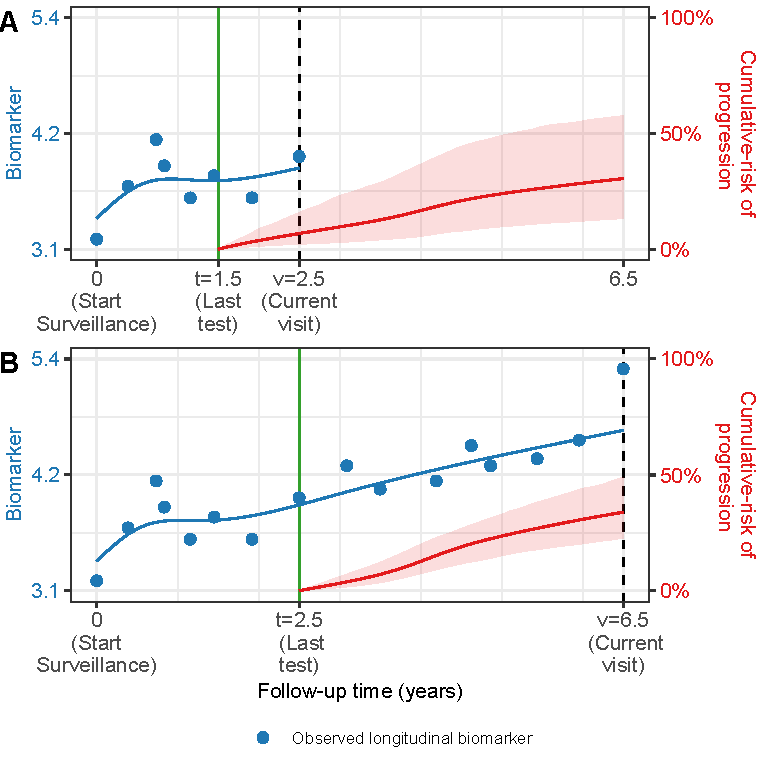
\includegraphics{contents/c4/images/c4_fig2.pdf}}
\caption{\textbf{Cumulative-risk of progression updated dynamically over follow-up} as more patient data is gathered. A single longitudinal outcome, namely, a continuous biomarker of disease progression, is used for illustration. \textbf{Panels~A,~B~and~C:} are ordered by the time of the current visit $v$ (dashed vertical black line) of a new patient. At each of these visits, we combine the accumulated longitudinal data (shown in blue circles), and time of the last negative invasive test $t$ (solid vertical green line) to obtain the updated cumulative-risk profile $R_j(u \mid t, v)$ (dotted red line with 95\% credible interval shaded) of the patient defined in~(\ref{c4:eq:cumulative_risk}). All values are illustrative.}
\label{c4:fig:2}
\end{figure}

\subsection{Personalized Test Decision Rule} 
\label{c4:subsec:pers_schedule}
We intend to exploit the cumulative-risk function $R_j(\cdot)$ to develop a risk-based personalized schedule of invasive tests for the $j$-th patient. Typically, invasive tests are decided on the same visit times on which longitudinal data (e.g., biomarkers) are measured. Let $U = \{u_1, \ldots, u_L\}$ represent a schedule of such visits (e.g., biannual PSA measurement in prostate cancer). Here, $u_1 = v$ is also the current visit time. The maximum future visit time $u_L$ can be chosen based on the available information in the training dataset $\mathcal A_n$. That is, tests for the new patient $j$ are planned only up to a future visit time $u_L$ at which a sufficient number of events in $\mathcal A_n$ are available for making reliable risk predictions (e.g., up to the 80\% or 90\% percentile of progression times).

We propose to take the decision of conducting a test at a future visit time $u_l \in U$ if the cumulative-risk of progression at time $u_l$ exceeds a certain risk threshold $\kappa$ (Figure~\ref{c4:fig:3}). In particular, the test decision at time $u_l$ is given by,
\begin{equation}
\label{c4:eq:personalized_decision_grid}
Q_j^\kappa (u_l \mid t_l, v) = I \big \{ R_j(u_l \mid t_l, v) \geq \kappa \big\}, \quad 0 \leq \kappa \leq 1,
\end{equation}
where $I(\cdot)$ is the indicator function, $R_j(u_l \mid t_l, v)$ is the cumulative-risk of progression at the current decision time $u_l$, and $t_l < u_l$ is the time of the last test conducted before $u_l$. Thus, the future time at which a test will be planned, depends on both the threshold $\kappa$ and the cumulative-risk of the patient. Moreover, when a test gets planned at time $u_l$, i.e., $Q_j^\kappa (u_l \mid t_l, v) = 1$, then the cumulative-risk profile is updated before making the next test decision at time $u_{l+1}$ (Figure~\ref{c4:fig:3}). Specifically, the cumulative-risk at time $u_{l+1}$ is updated by setting the corresponding time of the last test $t_{l+1}=u_l$. This accounts for the possibility that progression may occur after time $u_l < T^*_j$. Hence, the time of last test $t_l$ is defined as,
\begin{equation*}
t_l = \left \{ 
\begin{array}{ll}
t, & \mbox{if } l = 1,\\
u_{l-1}, & \mbox{if } l \geq 2 \mbox{ and } Q_j^\kappa (u_{l-1} \mid t_{l-1}, v) = 1,\\
t_{l-1}, & \mbox{if } l \geq 2 \mbox{ and } Q_j^\kappa (u_{l-1} \mid t_{l-1}, v) = 0.\\
\end{array}
\right.
\end{equation*}
We should note that in all future test decisions, we use only the observed longitudinal data up to the current visit time $v$, i.e., $\{\mathcal Y_{1j}(v), \ldots, Y_{Kj}(v)\}$.
\begin{figure}
\centerline{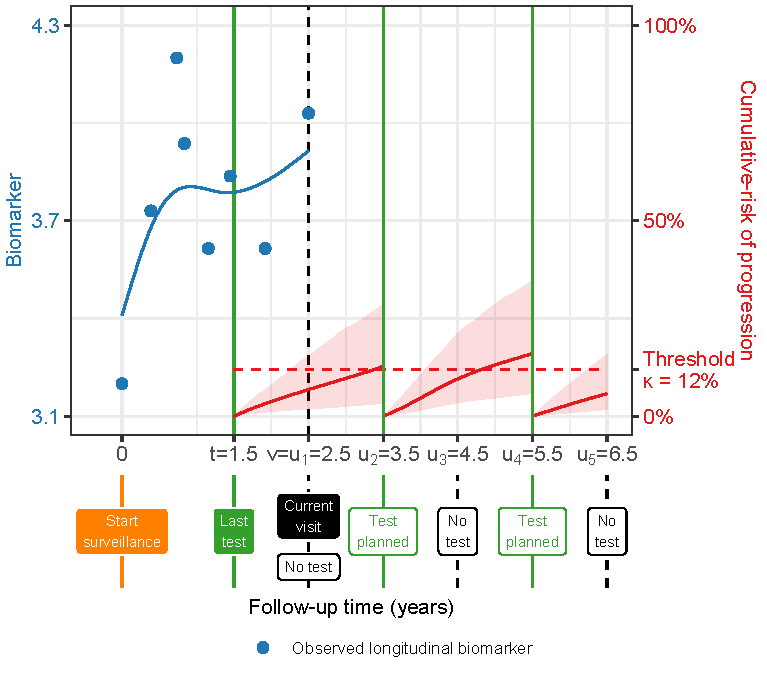
\includegraphics{contents/c4/images/c4_fig3.pdf}}
\caption{\textbf{Successive personalized test decisions based on patient-specific cumulative-risk of progression (\ref{c4:eq:personalized_decision_grid})}. Time of current visit: $v=2.5$ years (dashed vertical black line). Time of the last test on which progression was not observed: $t=1.5$ years. Longitudinal data up to current visit: $\mathcal{Y}_j(v)$ is a continuous biomarker (blue circles). Example risk threshold: $\kappa=0.12$~(12\%). Grid of future visits on which future tests are planned: $U = \{2.5, 3.5, 4.5, 5.5, 6.5\}$ years. The cumulative-risk profiles $R_j(u_l \mid t_l, v)$ employed in~(\ref{c4:eq:personalized_decision_grid}) are shown with dotted red lines (95\% credible intervals shaded), and are updated each time a test is planned (solid vertical green lines). Future test decisions $Q_j(u_l \mid t_l, v)$ defined in~(\ref{c4:eq:personalized_decision_grid}) are: $Q_j^\kappa(u_1=2.5\mid t_1=1.5,v)=0$, $Q_j^\kappa(u_2=3.5\mid t_2=1.5,v)=1$, $Q_j^\kappa(u_3=4.5\mid t_2=3.5,v)=0$, $Q_j^\kappa(u_4=5.5\mid t_2=3.5,v)=1$, and $Q_j^\kappa(u_5=6.5\mid t_5=4.5,v)=0$. All values are illustrative.} 
\label{c4:fig:3}
\end{figure}

\subsection{Expected Number of Tests and Expected Time Delay in Detecting Progression}
\label{c4:subsec:exp_delay_estimation}
To facilitate shared-decision making of invasive tests, we translate our proposed decision rule, i.e., the choice of a specific risk threshold $\kappa$, into two clinically relevant quantities. First, the number of tests (burden) we expect to perform for patient $j$, and second, if the patient progresses, the time delay (shorter is beneficial) expected in detecting progression. To calculate these two quantities, we first suppose that patient $j$ does not progress between his last negative test at time $t$ and the maximum future visit time $u_L$. Under this assumption, the subset of future visit times in $U$ on which a test is planned using~(\ref{c4:eq:personalized_decision_grid}) results into a personalized schedule of future tests (Figure~\ref{c4:fig:3}), given by:
\begin{equation}
\label{c4:eq:personalized_schedule_grid}
\{s_1, \ldots, s_{N_j}\} = \big\{ u_l \in U : Q_j^\kappa(u_l \mid t_l, v) = 1 \big\}, \quad N_j \leq L.
\end{equation}

If patient $j$ never progressed in the period $[t, u_L]$, as we initially supposed, all $N_j$ tests in $\{s_1, \ldots, s_{N_j}\}$ will be conducted. However, fewer tests will be performed if the patient did progress at some point $T_j^* < u_L$. We formally define the discrete random variable $\mathcal{N}_j$ denoting the number of performed tests in conjunction with the true progression time $T_j^*$ as,
\[
\mathcal{N}_j (S^\kappa_j) = \left \{
\begin{array}{ll}
1, & \mbox{ if } \; t < T^*_j \leq s_1,\\
2, & \mbox{ if } \; s_1 < T^*_j \leq s_2,\\
\vdots&\\
N_j, & \mbox{ if } \; s_{N_j-1} < T^*_j \leq s_{N_j},
\end{array}
\right.
\]
where $S^\kappa_j = \{s_1, \ldots, s_{N_j}\}$ is the schedule of planned future tests. The expected number of future tests for patient $j$ will be the expected value $E \big \{\mathcal N_j(S^\kappa_j)\big\}$, given by the expression,
\begin{equation*}
\label{c4:eq:exp_tests}
E \big \{\mathcal N_j(S^\kappa_j)\big\} = \sum_{n = 1}^{N_j} n \times \mbox{Pr}(s_{n-1} < T^*_j \leq s_n \mid T^*_j \leq s_{N_j}), \quad s_0 = t,
\end{equation*}
where 
\begin{equation*}
\mbox{Pr}(s_{n-1} < T^*_j \leq s_n \mid T^*_j \leq s_{N_j}) = \frac{R_j(s_n \mid t, v) - R_j(s_{n-1} \mid t, v)}{R_j(s_{N_j} \mid t, v)}.
\end{equation*}

Similarly, we can define the expected time delay in detecting progression, under the assumption that progression occurs before $u_L$. Specifically, the random variable time delay is equal to the difference between the time of the test at which progression is observed and the true time of progression $T_j^*$, and is given by,
\[
\mathcal D_j (S^\kappa_j) = \left \{
\begin{array}{ll}
s_1 - T_j^*, & \mbox{ if } \; t < T^*_j \leq s_1,\\
s_2 - T_j^*, & \mbox{ if } \; s_1 < T^*_j \leq s_2,\\
\vdots&\\
s_{N_j} - T_j^*, & \mbox{ if } \; s_{N_j-1} < T^*_j \leq s_{N_j},
\end{array}
\right.
\]
The expected time delay in detecting progression is the expected value of $\mathcal D_j (S^\kappa_j)$, given by the expression,
\begin{equation*}
\label{c4:eq:exp_delay}
E \big \{ \mathcal D_j(S^\kappa_j)\big\} = \sum_{n = 1}^{N_j} \Big\{s_n - E(T^*_j \mid s_{n-1}, s_n, v)\Big\} \times \mbox{Pr}(s_{n-1} < T^*_j \leq s_n\mid T^*_j \leq s_N),
\end{equation*}
where~$E(T^*_j \mid s_{n-1}, s_n, v)$ denotes the conditional expected time of progression for the scenario~$s_{n-1} < T^*_j \leq s_n$ and is calculated as the area under the corresponding survival curve,
\begin{equation*}
\begin{split}
E(T^*_j \mid s_{n-1}, s_n, v) = s_{n-1} + \int_{s_{n-1}}^{s_n} \mbox{Pr} & \Big\{T^*_j \geq u \mid s_{n-1} < T^*_j \leq s_n,\\ & \quad \mathcal{Y}_{1j}(v), \ldots, \mathcal{Y}_{Kj}(v), \mathcal{A}_n\Big\} \mathrm{d}u.
\end{split}
\end{equation*}

The personalized schedule in~(\ref{c4:eq:personalized_schedule_grid}), and the corresponding personalized expected number of tests and time delay, have the advantage of getting updated with newly collected data over follow-up. Also, the expected number of tests and time delay can be calculated for any schedule, fixed or personalized. Hence, patients/doctors can use them to compare different schedules. Although, a fair comparison of time delays between different schedules for the same patient, requires a compulsory test at a common horizon time point in all schedules.

\subsection{How to Select the Risk Threshold~$\kappa$}
\label{c4:subsec:kappa_selection}
The risk threshold $\kappa$ controls the timing and the total number of invasive tests in the personalized schedule $S^\kappa_j$. Through the timing and the total number of planned tests, $\kappa$ also indirectly affects the potential time delay (Figure~\ref{c4:fig:1}) in detecting progression if a particular schedule is followed. Hence, $\kappa$ should be chosen while balancing both the number of invasive tests (burden) and the time delay in detecting progression (shorter is beneficial).

To facilitate the choice of $\kappa$ in practice, following our developments in the previous section, we translate the different choices for threshold $\kappa$ into the expected number of tests and time delay. In particular, for a patient $j$ having data available up to his current visit time $v$, we can construct a bi-dimensional Euclidean space of his expected total number of tests (x-axis) and expected time delay in detecting progression (y-axis), for different personalized test schedules obtained by varying $\kappa$ in $[0, 1]$, e.g., Figure~\ref{c4:fig:4}.
\begin{figure}
\centerline{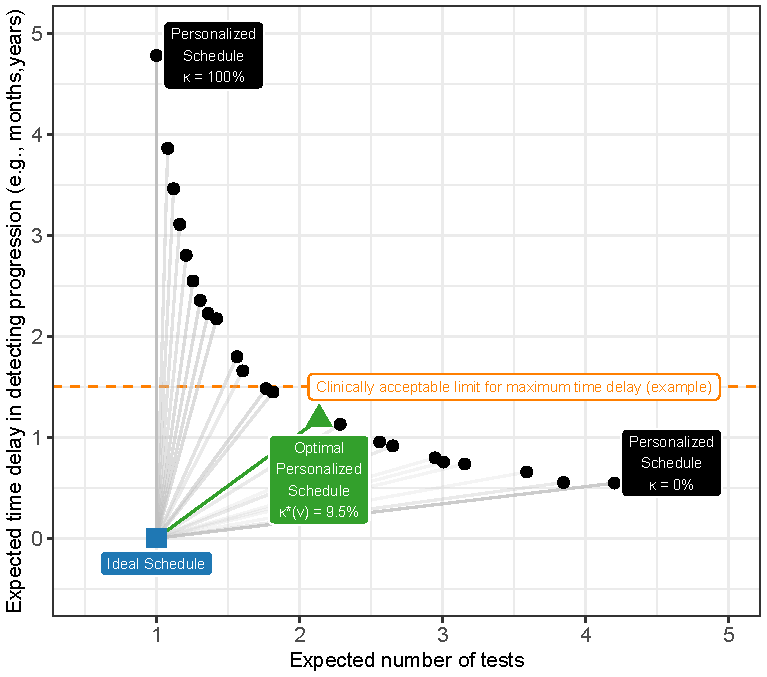
\includegraphics{contents/c4/images/c4_fig4.pdf}}
\caption{\textbf{Optimal current-visit time $v$ specific risk threshold $\kappa^*(v)$ obtained using~(\ref{c4:eq:kappa_choice})} for the patient shown in Figure~\ref{c4:fig:3}. Ideal schedule of tests: point (1,0) shown as a blue square. It plans exactly one invasive test at the true time of progression $T^*_j$ of a patient. Hence, the time delay in detecting progression is zero. Various personalized schedules based on a grid of thresholds $\kappa$ in $[0,1]$ are shown with black circles. Higher thresholds lead to fewer tests, but also higher expected time delay. The personalized schedule based on $\kappa^*(v)=9.5\%$ threshold (green triangle) has the least Euclidean distance (solid green line) to the ideal schedule. It is also possible to optimize the least distance under a certain clinically acceptable limit on the time delay (dotted horizontal orange line).}
\label{c4:fig:4}
\end{figure}

The ideal schedule for $j$-th patient is the one in which only one test is conducted, at exactly the true time of progression $T^*_j$. In other words, the time delay will be zero. If we weigh the expected number of tests and time delay as equally important, then we can select as the optimal threshold at current visit time $v$, the threshold $\kappa^*(v)$ which minimizes the Euclidean distance between the ideal schedule, i.e., point (1, 0) and the set of points representing the different personalized schedules $S^{\kappa}_j$ corresponding to various $\kappa \in [0, 1]$, i.e.,
\begin{equation}
\label{c4:eq:kappa_choice}
\kappa^*(v) = \argmin_{0 \leq \kappa \leq 1} \sqrt{\Big[E\big\{\mathcal N_j(S^\kappa_j)\big\} - 1\Big]^2 + \Big[E\big\{\mathcal D_j(S^\kappa )\big\} - 0\Big]^2}.
\end{equation}
In certain scenarios, patients/doctors may be apprehensive about undergoing more than a maximum expected number of future tests, or having an expected time delay higher than certain months. For such purposes, the Euclidean distance in ~(\ref{c4:eq:kappa_choice}) can be optimized under constraints on the expected number of tests or expected time delay (Figure~\ref{c4:fig:4}). Doing so alleviates two problems, namely, that the time delay and the number of tests have different units of measurement, and that in~(\ref{c4:eq:kappa_choice}) they are weighted equally~\citep{cook1994equivalence}.

We considered shorter delays in detecting progression as the benefit of repeated tests. However, it is also common to describe the benefit of testing in terms of decision-theoretic measures such as quality-adjusted life-years/expectancy (QALY/QALE) gained~\citep{sassi2006calculating}. Optimizing~(\ref{c4:eq:kappa_choice}) with QALE needs, setting the optimal point in a Euclidean space with QALE as a dimension, and obtaining expected QALEs for different schedules. For estimating the expected QALE in a personalized manner, a mathematical definition of QALE in terms of time delay~$\mathcal{D}_j$ in detecting progression~\citep{de2017should} is required.